\documentclass[a4paper,12pt]{article}
\pagestyle{plain}

\usepackage{graphics}
\usepackage{graphicx}
\usepackage{grffile}
\usepackage{epsfig}
\usepackage{rotating}
\usepackage{euscript}
\usepackage{eufrak}
\usepackage{color}
\usepackage{amsmath}
%\usepackage{amssymb}
\usepackage{multirow}  


\parindent      = 0.0in
\parskip        = 0.08in
\widowpenalty   = 10000
\clubpenalty    = 10000
\labelsep       = 0.1cm
\itemsep        = 0.0cm

\textheight 24cm
\textwidth  15cm
\oddsidemargin 0.in
\evensidemargin 0.in
\topmargin -0.25in
\footskip 0.75in
\headheight 0.in
\renewcommand{\bottomfraction}{1.0}
\renewcommand{\topfraction}{1.0}
\renewcommand{\textfraction}{0.0}

\def\st{\scriptstyle}
\def\sst{\scriptscriptstyle}
\def\mco{\multicolumn}
\def\epp{\epsilon^{\prime}}
\def\vep{\varepsilon}
\def\ra{\rightarrow}
\def\vp{{\bf p}}
\def\al{\alpha}
\def\ab{\bar{\alpha}}
\def\be{\begin{equation}}
\def\ee{\end{equation}}
\def\bea{\begin{eqnarray}}
\def\eea{\end{eqnarray}}

% Title Page
\title{First Year Report}
\author{Stefanie Lewis 0706250}


\begin{document}
\maketitle

\begin{abstract}
This PhD project focusses on the development of a modern analysis technique based on Bayesian statistics.  This analysis tool will eventually be used in the extraction of polarisation observables from data collected by the CLAS Collaboration in Hall B at Jefferson Lab, in Newport News, Virginia.  In this report, the familiarisation with various aspects of the PhD program, specifically software, will be discussed.  An introduction to the concept of nested sampling is included.  This idea of nested sampling, based on Bayesian analysis, is the basis of an alternative to maximum likelihood fitting.  The intermediary steps between a sample problem and a useful analysis tool will be discussed.  In the future, data collected from the excited nucleon (N*) program at CLAS will be analysed using this technique.  As such, a brief description of the surrounding theory is included - specifically baryon spectroscopy and pseudoscalar meson photoproduction.  The future work planned for this project is also discussed.  There is a clear plan for the further improvements and development of the nested sampling analysis tool.  There are plans to work in the future with the CLAS Collaboration on the tagger energy calibration for the g14 (HDIce) experiment in Hall B.  
\end{abstract}

\newpage
\tableofcontents

\newpage

\section{Introduction}
This PhD project is focused on the development of an analysis technique to be used in the extraction of polarisation observables in the N* program at CLAS. The results of such a tool can be used to develop a complete understanding of pseudoscalar meson photoproduction, which accesses the excited nucleon spectrum.  This would be used to find missing mass resonances, that is, mass resonances predicted by some quark models but not others.  The N* program at CLAS covers a wide spectrum of reactions which can be studied in order to gain a better understanding of the spin structure of nucleons \cite{nstar}.  Pseudoscalar meson photoproduction reactions are of particular interest.  These reactions provide an insight to the excited nucleon spectrum \cite{klempt}.   
\newline
%%%%EDIT THIS
Within the last 7 months, much time has been spent on getting accustomed to various aspects of the physics research environment.  Several new topics were explored; primarily Bayesian analysis (specifically Nested Sampling), object-oriented programming and baryon spectroscopy.  
\newline
A toy nested sampling program in C was provided \cite{sivia} and explored in order to become familiar with the algorithm.  The source code was then used to create a similar object-oriented program.  This provided an opportunity to not only introduce the concept of object orientation (specifically C++), but also to check the functional capabilities against those of the original C program.  Once the object-oriented program provided acceptable results, it was generalised in order to be applied to a variety of problems.  
\newline
The generalised program was then used to extract simplified spin observables from simulated data. This provided the opportunity to fine-tune the program and find any problems with the program. At this point, it was discovered that the program had an exceedingly long run-time when a high number of iterations were used, despite optimisation efforts.  The possibility of applying some of the programming techniques used in graphics processing units (GPUs) will be considered as a potential solution to the long run-time.
\newline
%Insert wee paragraph on shifts at JLab and various training exercises.
In addition to becoming accustomed to the computational skills, there has been some introduction to Jefferson Lab and the CLAS Collaboration.  A collaboration meeting in Paris was attended and a probationary membership to the collaboration has been approved.  Several training courses and exercises were done in preparation for shiftwork at Jefferson Lab's Experimental Hall B, including General Safety, Radiation Worker Safety and Oxygen Deficiency Hazard training.  



\section{Background}
\subsection{Baryon Spectroscopy and Spin Observables} 
%Baryon paper - Klempt, Richard
Despite the physics taught in undergraduate physics courses, the quark contributions to the spin of a nucleon are not well understood.  There exist several quark models which each attempt to provide an explanation of the spin nature of nucleons.  Baryon spectroscopy is an experimental approach used to support or preclude predicted quark models \cite{klempt}.  Each quark model predicts mass resonances at various energies in the nucleon spectrum.  There are some mass resonances, however, that are expected for some quark models and not others.  Finding these resonances that are missing from some quark models would exclude those models and provide a significant insight into the spin structure of the nucleon \cite{nstar, klempt}.
\newline
Pseudoscalar meson photoproduction is used to examine the spectrum of excited nucleon states.  The entire process of pseudoscalar meson photoproduction can be completely described by four complex amplitudes.  A beam of high-energy photons is directed onto a stationary nucleon target.  Mesons and the scattered nucleon are detected at points within the detector.  From the information detected, it is possible to extract various observables that can be linked to these four complex amplitudes.  There are, in total, fifteen observables (described in Table I), in addition to the differential cross-section, that can be extracted from variations in experimental set-up.  There are three single-spin observables - a photon-beam asymmetry ($B$), a recoil polarisation ($R$) and a target polarisation ($T$).  There are four beam-recoil ($BR$), four beam-target ($BT$) and four recoil-target ($RT$) spin polarisations.  These observables are all non-independent combinations of the four complex amplitudes.  As such, it is necessary to calculate multiple observables in order to extract the amplitudes. Data from suitably arranged experiments must be used to extract these observables \cite{nstar, info}.
\newline
%%%%This is from the Spin Observables section (which used to exist).  ABOVE HERE need to explain physics.
In order to become accustomed with the correlations and behaviour of spin observables, a small standalone program was created.  The aim of this macro was to generate dummy variables used to calculate the sixteen spin observables and output plots showing correlations between various observables.
\newline
Eight values were randomly generated from a Gaussian distribution over the surface of an 8-sphere.  These values were then combined to create four normalised complex amplitudes, $a_{1}$ to $a_{4}$.  Dummy values for these sixteen observables were calculated based on the expressions given in Table 1 below:
\newline
  \begin{center}
  \begin{table}[!h]
  \caption{Spin Observables in terms of Complex Amplitudes \cite{info}}
  \centering
  \begin{tabular}{c  c  c}
  \hline \hline
  Observable & Type & Amplitude Combination \\ [0.5ex]
  \hline \\
  $B$ & Single & $|a_{1}|^{2} + |a_{2}|^{2} - |a_{3}|^{2} - |a_{4}|^{2}$ \\
  $R$ & & $|a_{1}|^{2} - |a_{2}|^{2} + |a_{3}|^{2} - |a_{4}|^{2}$ \\
  $T$ & & $|a_{1}|^{2} - |a_{2}|^{2} - |a_{3}|^{2} + |a_{4}|^{2}$ \\ \\
  $E$ & Beam-target & $2\Re(a_{1}a_{3}^{*} + a_{2}a_{4}^{*})$ \\
  $F$ & & $2\Im(a_{1}a_{3}^{*} - a_{2}a_{4}^{*})$ \\ 
  $G$ & & $2\Im(a_{1}a_{3}^{*} + a_{2}a_{4}^{*})$ \\ 
  $H$ & & $-2\Re(a_{1}a_{3}^{*} - a_{2}a_{4}^{*})$ \\ \\
  $C_{x}$ & Beam-recoil & $-2\Im(a_{1}a_{4}^{*} - a_{2}a_{3}^{*})$ \\
  $C_{z}$ & & $2\Re(a_{1}a_{4}^{*} + a_{2}a_{3}^{*})$ \\
  $O_{x}$ & & $2\Re(a_{1}a_{4}^{*} - a_{2}a_{3}^{*})$ \\
  $O_{z}$ & & $2\Im(a_{1}a_{4}^{*} + a_{2}a_{3}^{*})$ \\ \\
  $T_{x}$ & Target-recoil & $2\Re(a_{1}a_{2}^{*} - a_{3}a_{4}^{*})$ \\
  $T_{z}$ & & $2\Im(a_{1}a_{2}^{*} - a_{3}a_{4}^{*})$ \\
  $L_{x}$ & & $-2\Im(a_{1}a_{2}^{*} + a_{3}a_{4}^{*})$ \\
  $L_{z}$ & & $2\Re(a_{1}a_{2}^{*} + a_{3}a_{4}^{*})$ \\ [1ex]
  \hline
  \end{tabular}

  \end{table}
  \end{center}
  %Insert table from Ireland's 
\newpage
Histograms were generated such that each observable was plotted against each other observable in order to determine any correlations between them.  

\begin{figure}[!ht]
 \begin{center}
  \includegraphics[scale=0.4]{histograms2D.eps}
  \caption{Observables were plotted against each other to show relationships between sets of observables.}
 \end{center}
\end{figure}

Plots showing circular patterns indicated that the two observables present in the histogram had a spherical correlation.  These have been documented in papers such as \cite{info, spin}. A significant number of plots showed rectangular patterns.  Pairs of observables that formed such a pattern were listed in order to find sets of three observables in which every possible pair constituted a rectangularly distributed histogram.  Thirteen such triples were found, and when plotted in three dimensions, formed a tetrahedron.

\begin{figure}[!h]
 \begin{center}
  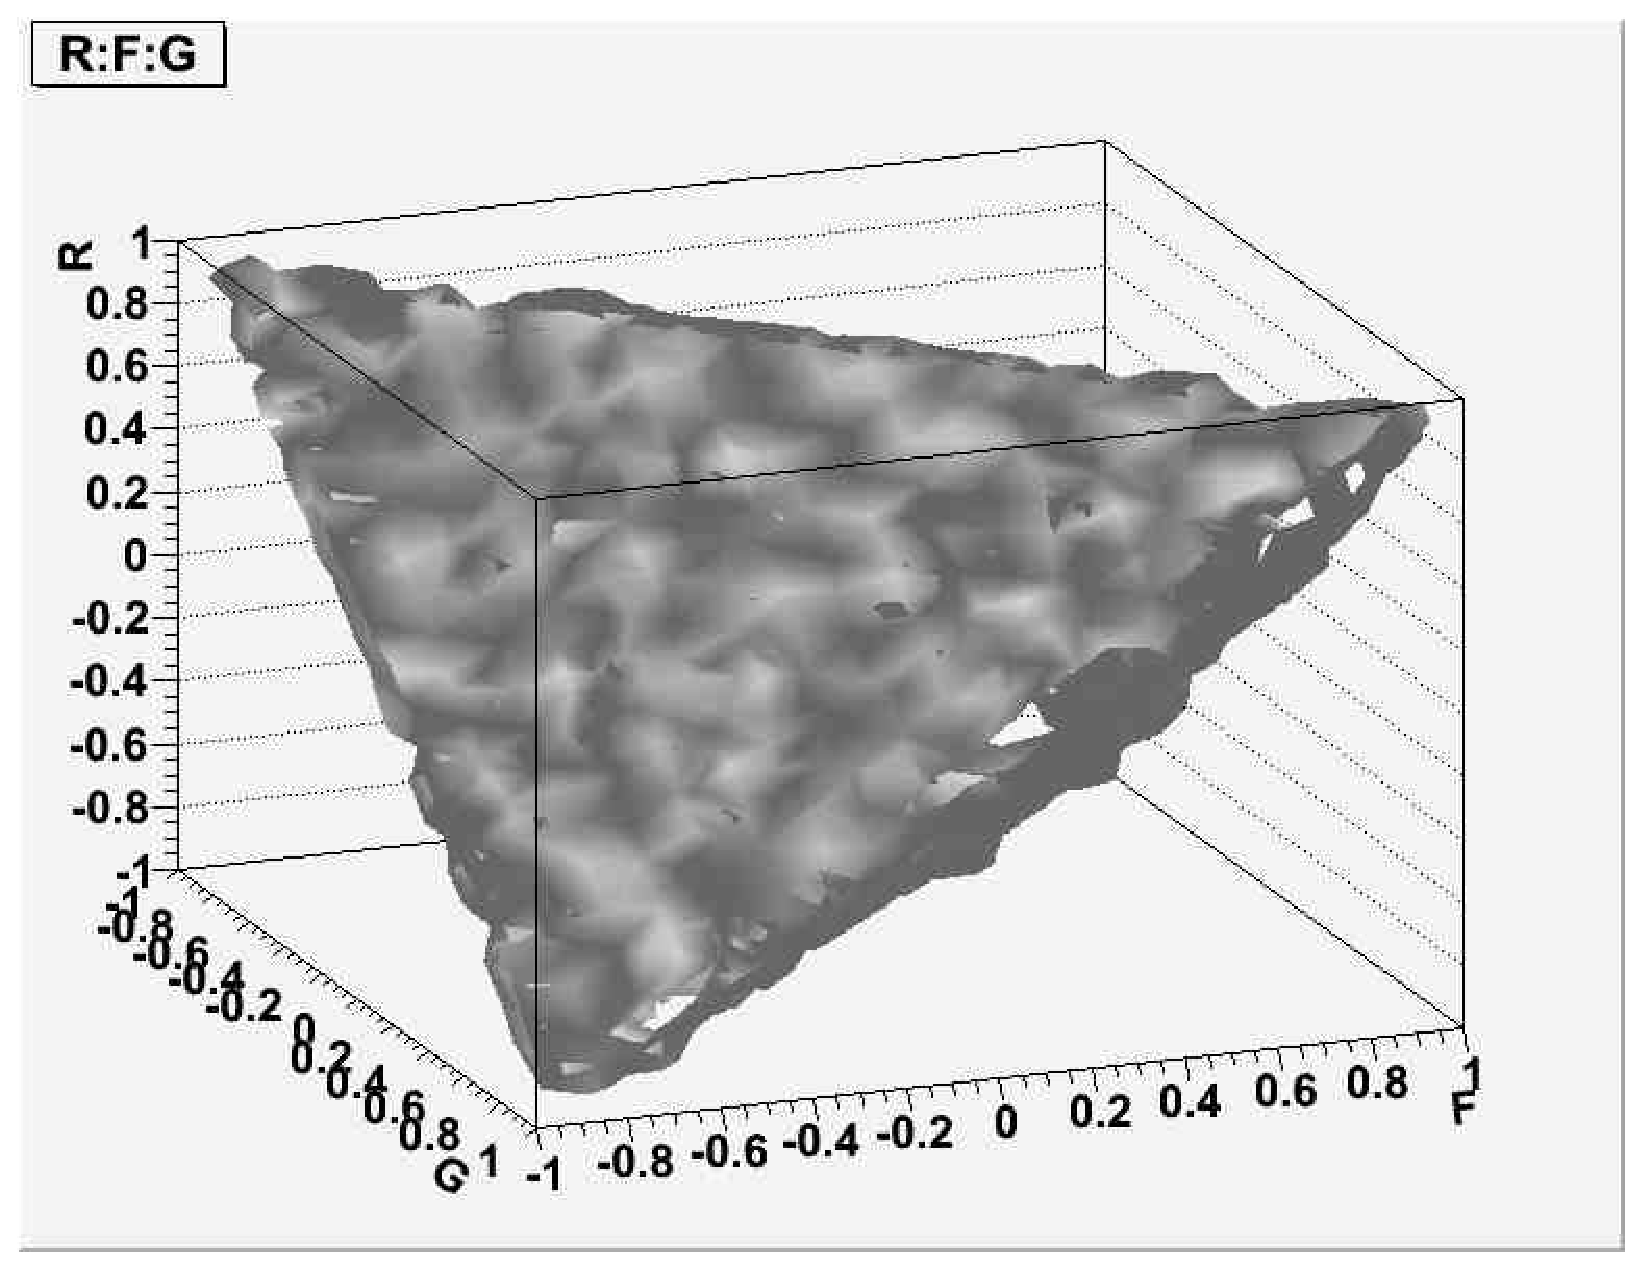
\includegraphics[scale=0.25]{RFG.eps}
  \caption{Tetrahedron resulting from plotting R, F and G in three dimensions.}
 \end{center}
\end{figure}

The equations defining the thirteen tetrahedra are shown in Figure 3.

\newpage
\begin{figure}[!ht]
 \begin{center}
  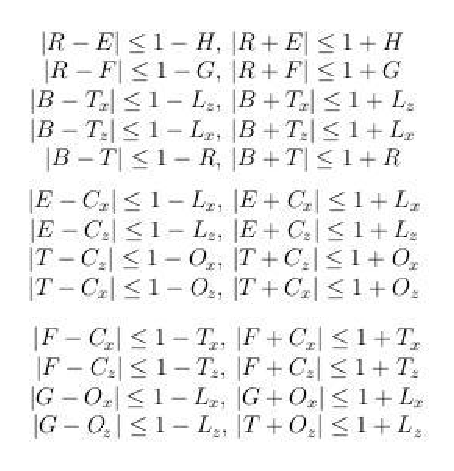
\includegraphics[scale=0.7]{ineqs.eps}
  \caption{The thirteen tetrahedral correlations correspond to the following triples: $REH, RFG, BT_{x}L_{z}, BT_{z}L_{x}, BTR, EC_{x}L_{x}, EC_{z}L_{z}, TC_{z}O_{x}, TC_{x}O_{z}, FC_{x}T_{x}, FC_{z}T_{z}, GO_{x}L_{x}$ and $GO_{z}L_{z}$.}
 \end{center}
\end{figure}

The significance of these thirteen triples is still being explored.
\newpage
\subsection{N* and CLAS at Jefferson Lab}
The CEBAF Large Acceptance Spectrometer (CLAS) Collaboration is based in Hall B of the Thomas Jefferson National Accelerator Facility (Jefferson Lab).  The CLAS detector has been used in many experiments.  Particularly relevant to this work is the N* (excited nucleon) program at CLAS \cite{clas}.  These highly excited nucleon states are used to gain a better understanding of quantum chromodynamics (QCD) as they are particularly sensitive to quark confinement \cite{nstar}.

The N* program encompasses a wide range of reactions, including several pseudoscalar meson photoproduction reactions, that are investigated to determine the quark structure of nucleons.  The specific reactions studied in this work can be described by the following equation:
\begin{equation}
 \gamma p \rightarrow K^{+} \pi^{-} p
\end{equation}
A high energy photon beam is incident on a stationary proton target.  The resulting pi mesons and the scattered proton hit the detector, which records values such as energy, position along detector and timing.  This information is then used to calculate more useful physical quantities, including mass, momentum and angular momentum distributions \cite{nstar}.  
\newline
The CLAS detector produces data in a raw form.  This data is then 'cooked' in order to present it in a useful format with the required data values.  A software package known as ROOTBEER, developed by Ken Livingston in Glasgow, is used to access information from these cooked data files \cite{rootbeer}.  This is a ROOT-based tool of bank event extraction routines.  
\newline
In the near future, CLAS will be undergoing a significant upgrade to CLAS12, where a higher energy beam (12 GeV from 6 GeV) will be installed.  This will enable the access of a large amount of data in regions where few experiments and collaborations are capable of exploring.  

\subsection{Nested Sampling}
%Sivia, Skilling
Nested sampling is a modern model comparison technique based on the principles of Bayesian statistics.  Most conventional analysis tools rely on the more widely known frequentist approach. In this approach, data is collected, and values such as the mean and standard deviation are extracted.  Any inferences are then based on the distribution of these statistics.  As such, the results are only based on a probability, and are not themselves probability statements.  The frequentist approach does not involve any knowledge or expectation of the results, and this is the key difference between frequentist and Bayesian statistics \cite{bayes}.
\newline
Bayesian statistics involves making an estimation of the results prior to any calculations.  This 'guess' is used to form a distribution with a easily determined mean and variance, known as the 'Prior'.  Bayes' Theorem (Eqn 2) is then used to combine the prior distribution with the data and produce a posterior distribution, the statistics of which determine the resulting mean, variance, etc \cite{sivia}. 
\newline

\begin{equation}
 prob(X|Y,I) = \frac{prob(Y|X,I) \times prob(X|I)}{prob(Y|I)}
\end{equation}
where I denotes any background information, X and Y are propositions, and $prob(X|Y,I)$ denotes the probability of X given Y and I.

The idea of Bayesian statistics can be expressed in the form of a simple equation \cite{skilling}:

\begin{equation}
 Prior \times Likelihood \longrightarrow Evidence \times Posterior
\end{equation}
where
\begin{equation}
 Prior = \pi(\theta)d\theta 
\end{equation}
\begin{equation}
 Likelihood = L(\theta)
\end{equation}
\begin{equation}
 Evidence = Z = \int LdX
\end{equation}
\begin{equation}
 Posterior = p(\theta)d\theta
\end{equation}

and
\begin{equation}
 dX = \pi(\theta)d\theta
\end{equation}

The prior is a distribution, or set of points that act as an initial starting point, an estimation or expectation of the results.  Each point has an associated likelihood determined by a likelihood function.  This is usually dependent on the applicable data.  For example, in an effort to determine the x-coordinate of an object, the prior would consist of a set of possible x-coordinates.  The likelihood associated with each point describes how likely that point is to be the x-coordinate of the object.
\newline
The output of a Bayesian calculation contains two pieces. The evidence, $Z$, is useful in comparing model assumptions.  Bayes factors, or ratios of evidence, are used to compare any two models at any time without the need to recalculate anything \cite{skilling}. The posterior is the distribution of points that result from the calculation.  These posterior points are determined primarily by the prior and likelihood.
\newline
Nested sampling is unique in that it extracts both parts of the Bayesian output.  For a specific problem, a prior is determined, as well as a problem-specific likelihood function.  Each point in the prior is assigned a likelihood value based on the likelihood function.  The nested sampling algorithm then finds the point with the lowest likelihood, i.e. the 'worst' point. A weight is determined for this worst point. Two values are then calculated - the natural log of the evidence, $log(Z)$, and the \textit{information} $H$, defined below \cite{sivia}.
\begin{equation}
 H = \int log(\frac{dP}{dX})dP
\end{equation}
where $dP$ is the posterior.  The values associated with the point - the point itself, its likelihood and its weight are all stored in the posterior.  The worst object is then overwritten with a copy of a 'surviving' point (any point other than the worst).  This copy is then slightly altered, usually by adding a small randomly generated number.  The likelihood of this 'new' point is then calculated and compared to that of the 'worst' object.  If it is found to be lower than the previously determined lowest likelihood, the new point is altered again.  This process uses a Markov Chain Monte Carlo (MCMC) to ensure that the resulting new point is only a slight change from a surviving point, and that its likelihood is at least higher than that of the overwritten 'worst' object.
\newline
This process is iterated through for either a predetermined number of iterates or until some termination condition is met \cite{skilling,sivia}.
\newline
The following diagram shows the process of nested sampling pictorially.  In this example, an object is placed at x = 3.  The prior consists of a set of x values distributed linearly on the interval (0,5).  The likelihood of the object being found at a given x-position is defined by the function below.
\begin{equation}
 L = 6x - x^{2} - 2
\end{equation}
The distribution of the points after each iterate of the nested sampling algorithm is shown in each line of the diagram below.


\begin{figure}[!h]
 \begin{center}
  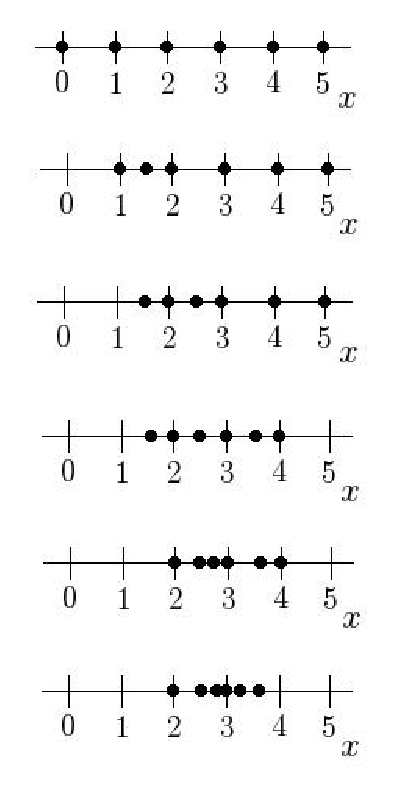
\includegraphics[scale=0.75]{nsdiagram.eps}
  \caption{After each iterate, the values begin converging on 3 - the position of the object.}
 \end{center}
\end{figure}

%Start by briefly describing the basic difference between the frequentist approach and Bayesian probability.
%Show equations used, in particular, Bayes' Theorem.
%Important to clearly explain all terms such as Prior, Posterior, Evidence, etc.

%This section could just follow on naturally from the last section, include equations and any diagrams that may help.
\newpage

\section{Nested Sampling}
\subsection{The Lighthouse Problem}
In order to become accustomed with both programming and the concept of Nested Sampling, a toy problem from \cite{sivia} was attempted: \\ \\
\textit{``A lighthouse is somewhere off a piece of straight coastline at a position $\alpha$ along the shore and a distance $\beta$ out at sea. It emits a series of short highly collimated flashes at random intervals and hence at random azimuths. These pulses are intercepted on the coast by photo-detectors that record only the fact that a flash has occurred, but not the angle from which it came. \textbf{N} flashes have so far been recorded at positions $x_{k}$. Where is the lighthouse?''} \cite{sivia}
\\ \\



\begin{figure}[!h]
 \begin{center}
  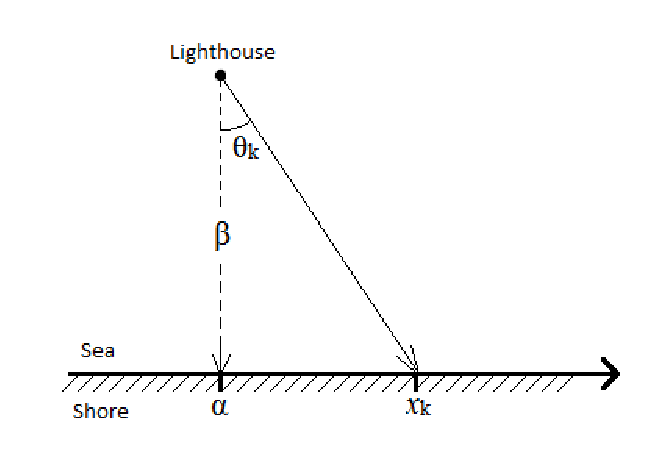
\includegraphics[scale=0.75]{lighthouse.eps}
  \caption{Diagram of Sivia's Lighthouse Problem \cite{sivia}}
 \end{center}
\end{figure}

\newpage
The 64 values of $x_{k}$ were previously generated with the lighthouse being positioned at (1,1) and were provided by \cite{sivia}.

Source code in C was provided and used to create an object-oriented program in C++.  The results of both approaches were compared and found to be equivalent, which ensured the functionality of the C++ version of the program.  The purpose of using object orientation was to ensure that the program was as generic as possible in order for it to be applied to other problems.  Several methods, however, were problem-specific.
\newline
     
The prior was assumed to be uniform on x = (-2,2) and y = (0,2).  That is, arrays of x and y coordinates were filled with values randomly generated on (0,1) and mapped to the intervals (-2,2) and (0,2) respectively.  Each (x,y) point was then used to calculate a likelihood value that reflected the probability of the lighthouse being situated at those coordinates.
\newline

\begin{equation}
 LogL = \sum log(\frac{(y/\pi)}{(D[k]-x)^{2} + y^{2}})
\end{equation}
where D is the array of flash positions $x_{k}$ and the expression is summed from k = 0 to 63.


%\newline 
The nested sampling algorithm is then run using the calculated likelihood values.  During each iteration, the Explore() function was called in order to overwrite the point with the lowest likelihood with an evolved copy of another point, as discussed in Section 2.3.  In this problem, small random numbers were added to the x and y values and a new likelihood was calculated.  If this new likelihood was less than that of the 'worst' object, it was rejected and the loop was run through again, with slightly larger random numbers added.  This loop, a Markov Chain Monte Carlo algorithm, was iterated twenty times in order to obtain a slightly altered copy of a surviving point with a likelihood greater than that of the overwritten point. 
\newline
The size of the prior (i.e. the number of samples used initially) and the number of iterates were altered in order to obtain an idea of the optimal set-up of the program.  The results of these tests are shown below.

%%%%%Insert no samples v no iterates

\begin{figure}[!h]
 \begin{center}
  \includegraphics[scale=0.5]{convergence.eps}
  \caption{Graph denoting the relation between number of objects (points) and number of iterates.  For each number of objects, the number of iterates at which the log of the evidence and the information were found not to change (i.e. the number of iterates required for them to converge) were plotted, respectively.}
 \end{center}
\end{figure}



Once a sufficient set of initial values was found, the results of the object-oriented program were compared to those obtained from the original C program.  The following plots show the comparison.  

%%%%%Insert results of both my code and Sivia's here.  Mention initial values in caption.  Also mention the position of the lighthouse (probably goes in a previous paragraph - where the data is mentioned).


\begin{figure}[!h]
 \begin{center}
  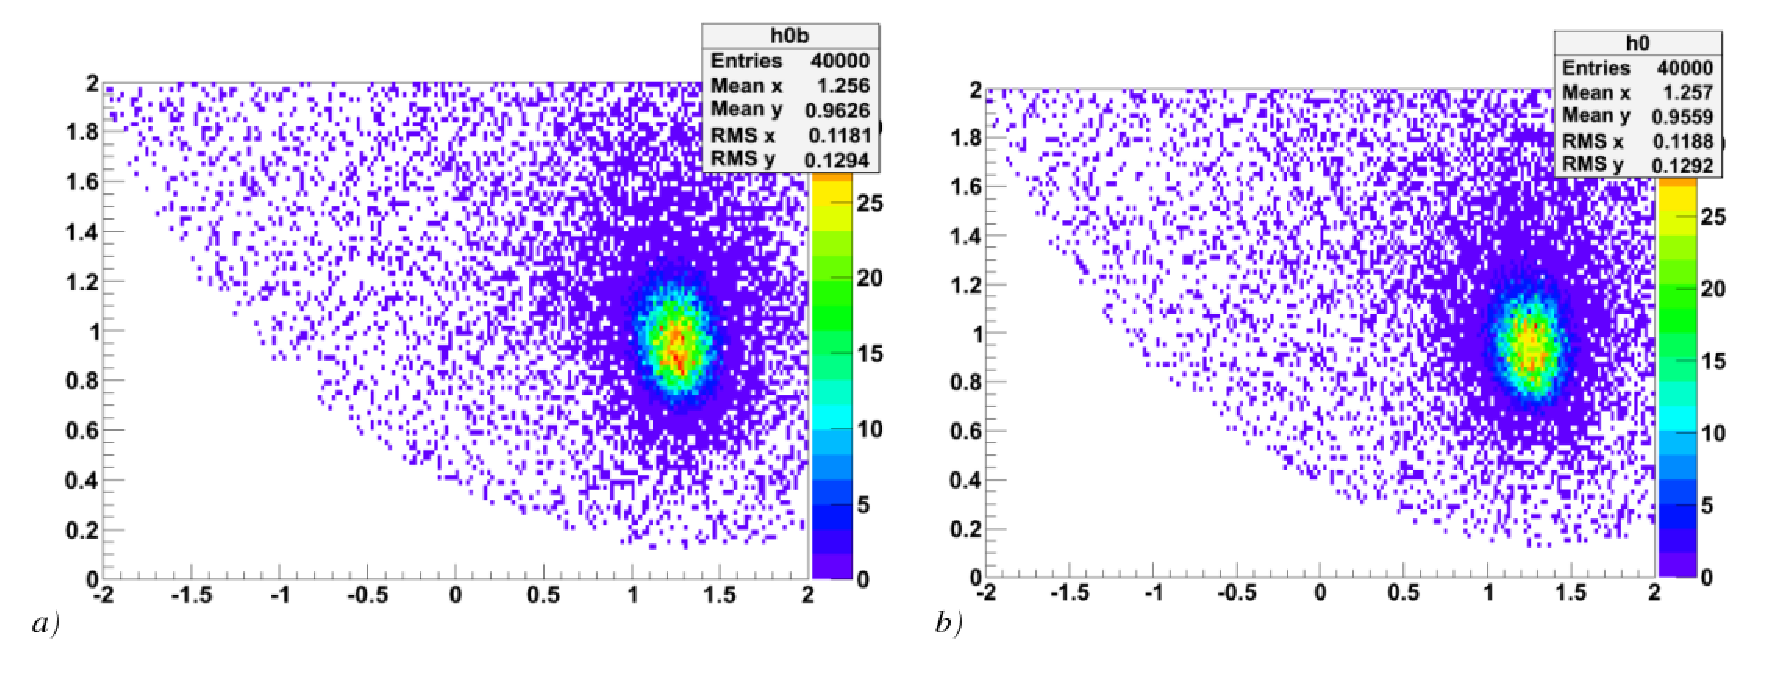
\includegraphics[scale=0.4]{lighthouseresults.eps}
  \caption{The results of running both versions of the code with the same initial values are shown above.  a) The C code provided by Sivia; b) The object-oriented C++ code.}
 \end{center}
\end{figure}

It was apparent from these plots that the two versions of the code were consistent with each other.  This test was used to ensure that the object-oriented version was functional to at least the same degree as the C code provided.  This was particularly useful in becoming familiar with programming in an object-oriented language.

\newpage
 
\subsection{Applications to Baryon Spectroscopy}
%Describe prior, likelihood and explore functions used in program.

%%%%Need to cite CLAS note.
Once a working version of the generic object-oriented nested sampling program was achieved, it was applied to a more physics-related problem.  The first task in this physics application was to extract the value of one observable - the photon-beam asymmetry, B (defined in Table I). An event generator was used to generate dummy data, given a specific value for B.  This data consisted of azimuthal angles and polarisation states.
%%%%Polarisation of what???
\newline
In this case, each point in the prior was described by eight normalised values randomly generated from a Gaussian distributed over the surface of an 8-sphere, in a similar manner as described in Section 2.1. %Spin observable section.
These values were then combined to form four complex transversity amplitudes, which were used to calculate a value of B based on the expression in Table I.  The likelihood associated with each calculated value of B was determined by the equations below \cite{dgi}.
\begin{equation}
 \tilde{A} = \frac{P_{\gamma}B\cos2\phi + \delta L}{1 + P_{\gamma}B\cos2\phi \delta L}
\end{equation}


\begin{equation}
X = \frac{1}{2}(1 \pm \tilde{A})
\end{equation}

\begin{equation}
logL = \sum log(X)
\end{equation}
where $P_{\gamma}$ is the photon polarisation number, $\delta L$ is the luminosity asymmetry and $logL$ is the natural logarithm of the likelihood.  In Eqn. 13, %Middle one!
$\tilde{A}$ was added or subtracted based on whether the associated polarisation was perpendicular or parallel, respectively.  These values were summed for all events - that is, all angles and polarisation states.  
\newline
These values were then used as usual in the nested sampling algorithm.  The Explore() function added a small randomly generated number to each of the eight initial values.  The small randomly generated number was determined by a Gaussian distribution of a set width.  This width was altered after each iteration of the MCMC loop in the function.  As per the Lighthouse example described in Section 3.1, a new likelihood value was calculated and compared to that of the 'worst' point in order to ensure that the new point was at least more likely than that which had been overwritten.  The results of the program were compared to the value of B input into the event generator.

%%%%%Insert results plots here.  Mention in caption number of iterates and samples.

\begin{figure}[!h]
 \begin{center}
  \includegraphics[scale=0.25]{B_3000_40000.eps}
  \caption{Resulting value of B after running the program with 3000 samples and 40 000 iterations.}
 \end{center}
\end{figure}


\subsubsection{Updated Prior}
%Describe evolved prior.  Need plots showing how prior and results evolve each time.
%Describe algorithm, show equations.
It was possible to add some complexity to the simple observable extraction program by using a previously generated posterior to confine the prior.  This would be particularly useful in the case where two or more measurements have been taken: in order to reduce the number of iterations required to achieve a precise result, the posterior of the initial measurement can be used to create a restricted prior.  The posterior generated by the program contained tens of thousands of points (determined by the number of iterations) with unequal weights.  It was found that these points contained in the posterior could be used to generate a more accurate prior, rather than using random numbers from a Gaussian distribution on the surface on an 8-sphere.  A ``cumulant staircase'' was used to create an equally-weighted posterior \cite{sivia}.
%Insert diagram of cumulant staircase here.

\begin{figure}[!h]
 \begin{center}
  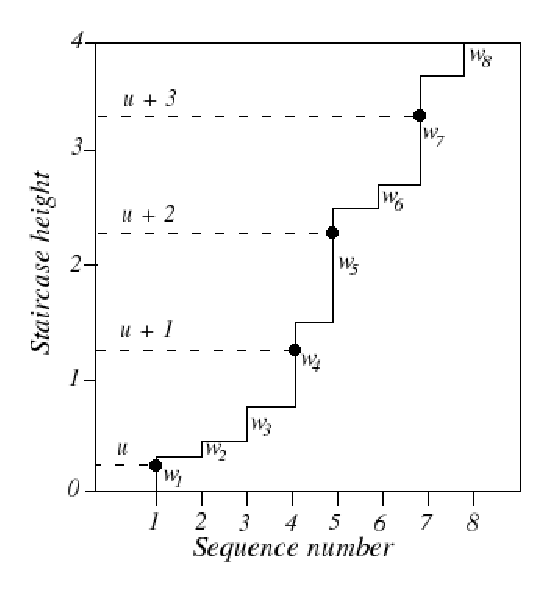
\includegraphics[scale=1]{staircase.eps}
  \caption{Cumulant staircase, describing the extraction of four equally weighted points from an unequally weighted posterior consisting of 8 points \cite{sivia}.}
 \end{center}
\end{figure}

The following equation was used to create equally weighted samples.  
\begin{equation}
 S_{k} = u + \nu \sum_{j=1}^{k} w_{j}
\end{equation}
where $S_{k}$ is the height of stair \textit{k}, $u$ is a random number generated from a distribution uniform on (0,1), $\nu$ is the number of equally weighted samples required and $w_{j}$ are the weights of the samples in the posterior.
\newline
Whenever this $S_{k}$ just exceeded an integer, the current point in the posterior was added to the new prior distribution.  

In this method, $\nu$ samples were drawn from the posterior.  A limit was applied to the number of samples that could be withdrawn in order to prevent repetition.
\begin{equation}
 \nu \leq \frac{1}{max_{k} (w_{k})}
\end{equation}

%Describe method and equation.
This updated (or evolving) prior has provided promising results, although tests on this section of the program are still ongoing.

\section{Analysis Program}
\subsection{SCons}
In the CLAS Collaboration at Jefferson Lab, a software construction tool called SCons \cite{scons} has become increasingly popular.  It is a simple, relatively easy-to-use alternative to the more commonly used Makefile.  The nested sampling program developed in this project was compiled using this SCons program.  SCons is scripted using Python, and is thus fairly intuitive to code.  The main file, required to be named 'sconstruct', imported any required Python scripts, listed the source code files to be compiled and any compiler flags required. Several Python scripts were imported in order to compile using ROOT libraries.  This provided a straightforward alternative to the complicated standard, autoconf.


 
\subsection{Structure and Coding}
An object-oriented (specifically C++) approach to the program was taken in order to make the nested sampling algorithm as generic as possible.  The program was comprised of two main classes, with a third acting as the user's front end (where various changes can be made). A combination of C++ and ROOT libraries were used.  
\newline

\begin{figure}[!h]
 \begin{center}
  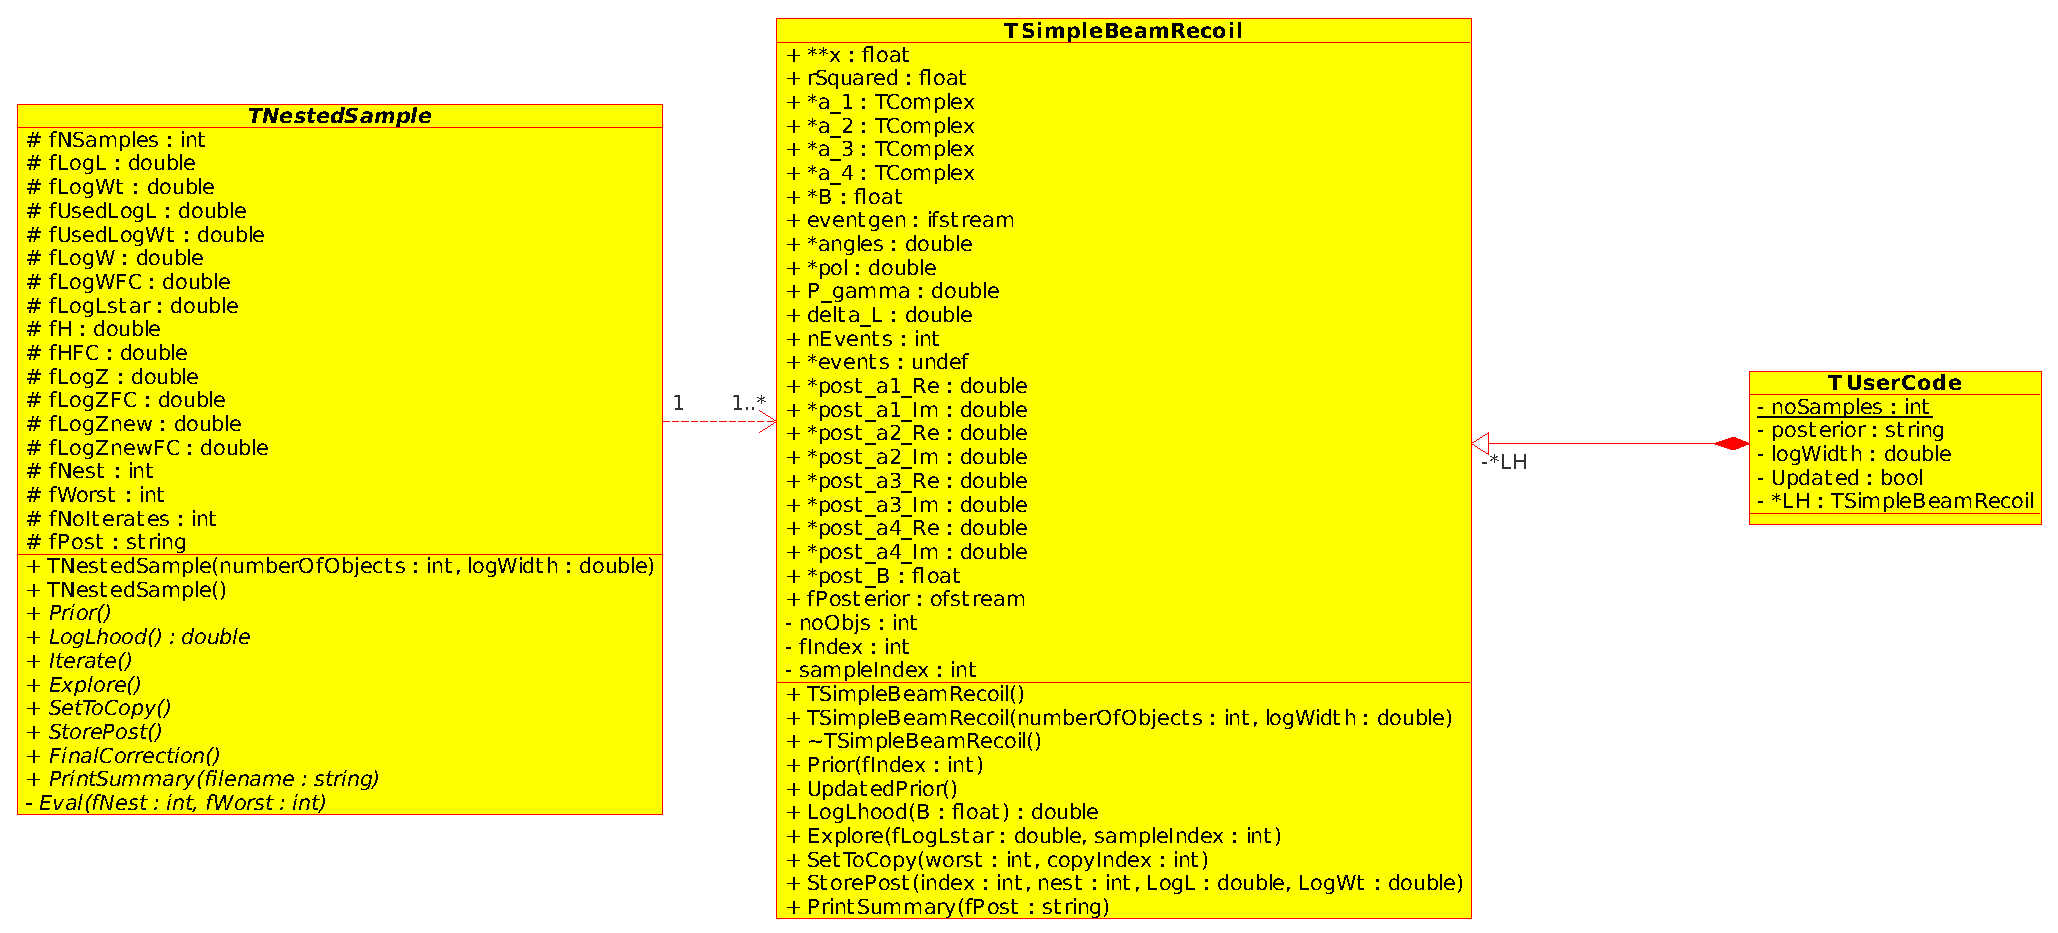
\includegraphics[scale=0.5]{class_diagram.eps}
  \caption{Class diagram showing methods, attributes and associations.}
 \end{center}
\end{figure}

An abstract class, TNestedSample, was used for defining the generic methods - Iterate(), Eval() and FinalCorrection().  These methods are responsible for the iteration over the nested sampling algorithm, termination and the nested sampling algorithm itself.  Other methods, such as Prior(), Explore() and PrintSummary(), must be defined for each derived class (i.e. for each application) as they are problem-specific.  The front end class, called TUserCode, determined which derived class would be used, called all required functions and set some initial values.  In principle, one could have multiple derived classes (i.e. applications to different problems) in one directory, and the user would be able to specify in TUserCode which derived class to use.  Each derived class would inherit the generic methods from the parent class.  For example, both Sivia's Lighthouse problem and the application to simple B observable extraction used the same abstract parent class - they differed solely in the derived classes.  
\newline
The nested sampling algorithm was contained in the Eval() method.  This private method was called from within the Iterate() method, which determined the number of iterations required in order to ensure a sufficiently precise result. A termination condition was determined based on work by Skilling \cite{skilling}.

%%%%%%%% Talk about termination condition here.

This termination condition ensured that the values for Log(Z) (the natural log of the evidence) and the information, H, differed only by a small amount respectively between iterations.  This could be written as ``The number of iterates should significantly exceed the product of the number of samples and the information H'' \cite{skilling}.
\newline
In the program, this condition was implementing in a for loop as shown below:
\newline
\begin{verbatim}
 for (fNest = 0; fNest <= N*fNSamples*fH){
      // run code
  }
\end{verbatim}
where fNest is the number of iterations, fNSamples is the number of samples, fH is the information and N is an integer whose value can be changed.  

%\newline
An small, additional method was implemented called FinalCorrection().  This was intended to be an optional small correction to the calculations.  This method went through the samples, determined a log weight for each (much in the same way as in the core nested sampling algorithm - but did not require the program to find the point with the lowest log-likelihood) and calculated Log(Z) and H as normal.  The Explore() function was not called from this method as the samples were not changed.  The results were stored in the posterior as before.  


%%%%% Show termination condition plots here

\subsection{Output}
The nested sampling program generated an output in several forms.  Basic information about the running of the program was output to the screen, as shown in Figure 3.
%Insert wee screenshot of basic output to terminal.

\begin{figure}[!h]
 \begin{center}
  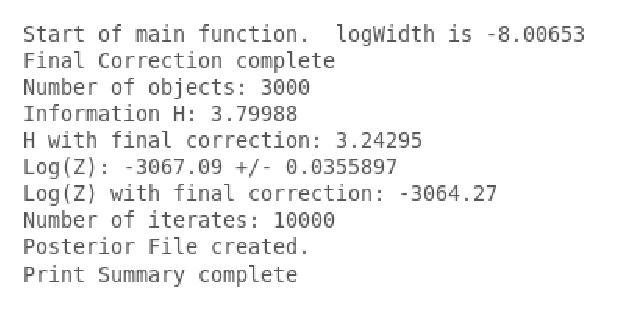
\includegraphics[scale=0.8]{term_output.eps}
  \caption{Information shown in terminal after running TSimplePhysics program.}
 \end{center}
\end{figure}

The standard deviation uncertainty for Log(Z) was printed (as shown in Fig. 4) based on the following equation provided by Sivia \cite{sivia}:
\begin{equation}
 \sigma = \sqrt{\frac{Information\  H}{Number\  of\  samples}}
\end{equation}


%Maybe briefly describe the terms that are output?
In addition to outputting to the screen, a ROOT tree (written to a .root file) was also created.  This tree was used to store many types of information in the form of branches.  The ROOT tree was used to examine the results visually.  A ROOT macro was written and used to generate several histograms showing the key results from the posterior.  Examples of these plots can be found in Sections 3.1 and 3.2.


During testing of the program, additional text files were output in order to ensure that various sections of the code were working as intended.  In particular, the introduction of an evolved prior required several files to be created and examined in ROOT.


\subsection{Performance Testing}
Several performance tests were carried out on the program in order to determine its ability to extract the desired observables.  All tests were done using data simulated by an event generator provided.  An input value of the spin observable, B, was set and the event generator produced data in both perpendicular and parallel polarisations.  This data was applied to the likelihood function of the program and the results were compared to the initial input values.
\subsubsection{Termination Condition Tests}
The termination condition suggested by Skilling \cite{skilling} contained a variable, $N$, that could essentially be used to set the desired precision of the results.  This parameter determined by how much the number of iterations exceeded the product of the number of samples and the information.  As $N$ was increased, the precision of the program also increased, as did the amount of time required for computation (see Section 4.3).  For this reason, it was important to determine a value of $N$ that allowed for the program to be sufficiently precise but also did not require an excessive amount of time to run.  In the case of the TSimplePhysics program described above, values of approximately 2-5 were found to be effective.

%%% Insert plots here.

\begin{figure}[!h]
 \begin{center}
  \includegraphics[scale=0.35]{logZplot.eps}
  \caption{Plot showing the convergence of Log(Z) and the values obtained at N = 2.}
 \end{center}
\end{figure}


\begin{figure}[!h]
 \begin{center}
  \includegraphics[scale=0.4]{Hplot.eps}
  \caption{Plot showing the convergence of H and the values obtained at N = 2.}
 \end{center}
\end{figure}


\begin{figure}[!h]
 \begin{center}
  \includegraphics[scale=0.4]{term_cond.eps}
  \caption{Plot showing relation between value of N and number of iterations performed.}
 \end{center}
\end{figure}
\newpage
\subsubsection{Timing Tests}
%Describe timing tests and implications.  GPU possibility here!!
During the above tests, it was found that the program took an excessive amount of time to run with any decent amount of precision.  The time required to run the program with different number of iterations of the nested sampling algorithm was recorded and plotted against the number of iterations. 

%%% insert timing plot here

\begin{figure}[!h]
 \begin{center}
  \includegraphics[scale=0.5]{timing.eps}
  \caption{Time required to run program with various numbers of iterations.}
 \end{center}
\end{figure}


The amount of time required for the program to run was decided to be significantly greater than desired.  At this point, the potential use of graphics processor unit (GPU) processing and data parallelisation was suggested.  This path is still currently being investigated.  

\newpage

\section{Summary}
Over the past seven months, there has been much work done in order to become familiar with the theory and the software used in the field. Nested sampling proved to be a significant portion of this work.  Initially, a toy problem was examined in which the location of a lighthouse was determined based on the positions of flashes along a coastline.  The source code for this example was provided in C.  The code was then adapted to C++ to allow for an object-oriented approach to be taken.  This object-orientation resulted in a nested sampling program that could be applied to many problems relatively simply.  Various tests were performed on the program to determine its accuracy to known results and to explore the effects of changing the initial parameters. Several ROOT macros were created for the generation of output plots.  Once it was shown that the program was functioning reasonably, the nested sampling program was applied to a simplified pseudoscalar meson photoproduction analysis in which the photon-beam asymmetry ($B$) was extracted.  A suitable prior and likelihood function were determined based on information found in literature.  An event generator was provided in which an initial value of $B$ was chosen and sample data was created.  This data was then applied to the program and the results produced were compared to the values input into the event generator.  The number of iterations of the nested sampling algorithm required for sufficiently accurate and precise results was determined and a termination condition was explored.  Through these performance tests, it was found that the program required significantly more time to run than anticipated.  Even after attempts to optimise the code, the amount of time for the program to run was excessive.  This became a notable setback.  Potential solutions to this problem are still being explored, in particular the use of GPU (graphics processor unit) processing and data parallelisation.  Concurrently, attempts were made to create an updated prior.  In this situation, a new, non-random equally weighted prior was determined from an unequally weighted posterior created from a previous run of the program.  The effectiveness of this updated (or evolving) prior is still being determined.
\newline
An introduction to the CLAS Collaboration also contributed to the work done during this first year.  Basic training was performed at Jefferson Lab in Newport News, Virginia.  Simple tasks were undertaken to become familiar with various aspects of data analysis at the lab.  These included a brief introduction to ROOTBEER and learning how to retrieve raw and cooked data from tape silos.  

\newpage

\section{Future Work}

Despite promising results, there is still much work to be done in the development of this Nested Sampling analysis program.  In the next twelve months, the program will be improved through a number of amendments.  Initially, the nested sampling program was simple and basic.  The level of complexity has been (and will continue to be) increased until it can be run on experimental data.  
The first step in this development is to handle all observables.  Instead of simply extracting the B observable, all sixteen observables will be extracted.  Calculations of statistical errors must also be included in the program.

Once this improvement has been implemented, it will be tested with data from experiment that has previously been studied.  The results will be compared to those obtained from a maximum-likelihood analysis program in order to ensure an acceptable level of accuracy. Once a sufficient degree of accuracy has been shown (and any necessary tweaks and adjustments have been made), the program will be used to evaluate new experimental data.

One of the drawbacks of this nested sampling approach is the excessive run-time required to obtain good results.  As discussed previously, this poses a significant problem.  The amount of time required to run the program using a sufficient number of iterations is longer than desired, despite optimisations.  The possibility of applying programming techniques used in graphics card programming and graphics processing unit (GPU) programming, in particular data parallelisation, will be strongly considered.  If successful, this would dramatically reduce the amount of time required to run the program with a high number of iterations. The implications of this improvement could enable the program to handle exceptionally large data sets in just minutes, making it a more desirable alternative to maximum likelihood methods.

There will also be some involvement in the g14 (HDice) experiment at CLAS at Jefferson Lab. This project would be specific to the tagger energy calibration.  Any discrepancies in the tagger required to determine the photon energy must be found and calibrated to produce meaningful data.  This will involve using ROOTBEER, a ROOT-based program developed by Ken Livingston.  In order to perform this task, some time will also be spent becoming familiar with the software and various aspects of acquiring data files from the CLAS tape silos and farms. 


\begin{thebibliography}{99}
%biblio
\bibitem{nstar} I. Aznauryan, V. Burkert, T.-S. Lee, V. Mokeev, arXiv:1102.0597v3 [nucl-ex], February 2011
\bibitem{klempt} E. Klempt, J.-M. Richard, Rev. Mod. Phys. 82, 1095-1153 (2010)
\bibitem{sivia} D. Sivia and J. Skilling, \textit{Data Analysis - A Bayesian Tutorial.} 2nd ed. Oxford Science Publications (2006)
\bibitem{info} D. G. Ireland, Phys. Rev. C 82, 025204 (2010)
\bibitem{spin} X. Artru, J.-M. Richard, J. Soffer, Phys. Rev. C 75, 024002 (2007)
\bibitem{clas} V. D. Burkert, Nucl. Phys. A 684, 16-25 (2001)
\bibitem{rootbeer} K. Livingston, University of Glasgow Nuclear Physics Group, 2004. \textit{ROOTBEER}. [online] Available at: \textless http://nuclear.gla.ac.uk/~kl/rootbeer/index.php \textgreater [Accessed 28 April 2011]
\bibitem{bayes} D. J. Bartholomew, Biometrika 52 (1-2), 19 (1965)
\bibitem{skilling} J. Skilling, Bayesian Analysis 1 4, 833 (2006)
%\bibitem{bayes} D. J. Bartholomew: A Comparison of Some Bayesian and Frequentist Inferences. Biometrika Issue 4 833-860, 2006
\bibitem{dgi} D. G. Ireland, Internal notes.
\bibitem{scons} The SCons Foundation, 2004. \textit{SCons: A Software Construction Tool.} [online] Available at: \textless http://www.scons.org \textgreater [Accessed 20 January 2011]
\end{thebibliography}

\end{document}          
